\chapter{Auswertung}

Im folgenden Kapitel wird die Auswertung anhand der in Kapitel (X) aufgestellten Bewertungskriterien beschrieben. Zu den einzelnen Kategorien (siehe Kapitel (X)) wird der jeweilige ausgefüllte Abschnitt der Bewertungsmatrix dargestellt und erläutert. 

\section{Kosten und Lizenz}

Nachfolgende Abbildung (X) zeigt den Abschnitt 'Kosten und Lizenz' der ausgefüllten Bewertungsmatrix.

\begin{figure}[h]
	\centering
	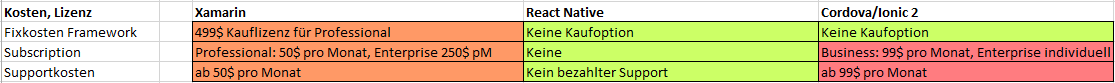
\includegraphics[width=1\textwidth]{Bilder/Auswertung_KostenLizenz.PNG}
	\caption{Bewertungsmatrix Kategorie Kosten und Lizenz}
	\label{fig:AuswKostLiz}
\end{figure}

Das Xamarin Framework gibt es in einer kostenlosen Community-Version und in den kostenpflichtigen Versionen 'Professional' und 'Enterprise'. Die kostenlose Community-Version gibt es für Windows inklusive einer Community-Version von Visual Studio und für Apple mit der IDE 'Xamarin Studio'. Die Preise der kostenpflichtigen Versionen richten sich nach den Preisen der entsprechenden Version der IDE Visual Studio. Die Professional-Version kann für 499\$ ohne Subscription oder für 1199\$ mit Subscription erworben werden. Eine Subscription hält 2 Jahre, ein Auffrischen danach kostet 799\$. Die Enterprise-Version kann nur mit Subscription erworben werden. Sie kostet 5999\$ und ein Auffrischen nach Ablauf der 2 Jahre kostet 2569\$. Einen technischer Support  erhält man mit jeder Subscription, das bedeutet ab umgerechnet 50\$ pro Monat. E-Mail-Support erhalten alle Business- und Enterprise-Kunden. Zusätzlich zu allen Modellen kann die Xamarin Test-Cloud ab einen monatlichen Preis von 99\$ genutzt werden.
\\
\\
Für das Framework React Native gibt es keine kostenpflichtigen Versionen. 
\\
\\
Für das Framework Cordova gibt es ebenfalls keine kostenpflichtigen Modelle. Das Framework Ionic bietet dagegen folgende Varianten an: eine kostenlose Community-Version und die kostenpflichtigen Versionen 'Indie', 'Business' und 'Enterprise'. Im Gegensatz zu den kostenpflichtigen Modellen bei Xamarin, fallen bei den Modellen von Ionic monatliche Subscription-Gebühren an. Die Indie-Variante kostet 25\$ pro Monat und die Business-Variante kostet 99\$ pro Monat. Für die Enterprise-Version gibt es einen individuellen Preis auf Anfrage. Ab der Business-Variante erhält man E-Mail-Support, das bedeutet ab 99\$ pro Monat. Möchte man die Ionic Test Cloud nutzen, so kostet dies 20\$ pro Monat und Anwendung.  

\section{Support und Community}

\section{Entwicklung}

Die ausgefüllte Bewertungsmatrix für die Kategorie 'Entwicklung' ist in nachfolgender Abbildung (X) dargestellt.

\begin{figure}[h]
	\centering
	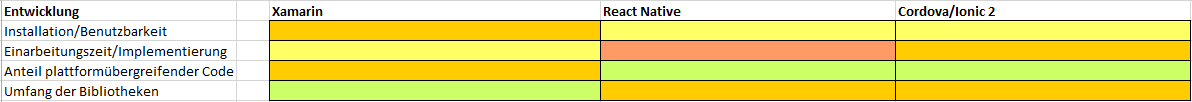
\includegraphics[width=1\textwidth]{Bilder/Auswertung_Entwicklung.PNG}
	\caption{Bewertungsmatrix Kategorie Entwicklung}
	\label{fig:AuswEntw}
\end{figure}

Hat man bereits ein Visual Studio installiert und möchte Xamarin integrieren, so ist dies nicht ohne Mehraufwand möglich. Einfacher ist es, Visual Studio direkt zusammen mit Xamarin zu installieren. Hierzu muss nur der Installer von der Xamarin Homepage heruntergeladen und ausgeführt werden. Alles Notwendige für die Entwicklung mit Xamarin ist bei der Installation von Visual Studio bereits vorausgewählt. Der Xamarin Installer installiert zusätzlich noch weitere benötigte Komponenten, wie ein Android SDK und NDK. Es muss keine weitere Software separat beschafft werden. Startet man nach der erfolgreichen Installation die IDE Visual Studio, so kann direkt mit der Entwicklung mit Xamarin gestartet werden, indem ein neues Projekt 'Android App' angelegt wird. Anders als bei der nativen Entwicklung mit Android Studio gibt es hier allerdings keine Design-Vorauswahl bei der Projekterstellung wie zum Beispiel einen \textit{NavigationDrawer} für die Navigation. Dafür gibt es sogenannte 'Pre Built Apps', das sind beispielhafte fertige Anwendungen, wie unter anderem Shopping- oder CRM-Anwendungen. 
\\
Auf der Xamarin Homepage findet sich einiges an Beispielcode zu verschiedensten Funktionalitäten. Viele dieser Beispielprojekte sind allerdings nicht direkt kompilierbar. Es ist immer aufwendiges recherchieren notwendig, welche Verweise, Components oder Einstellungen im Projekt angepasst werden müssen, da diese Informationen nicht mit angegeben sind. Für die Verwendung von zum Beispiel nativen UI-Elementen müssen sogenannte 'Components' installiert und dem Projekt hinzugefügt werden. Welche 'Components' für ein gewünschtes Feature benötigt werden muss selbst recherchiert werden. Bei der Auswahl dieser 'Components' gibt es oft Schwierigkeiten, da manche 'Components' zwingend in einer übereinstimmenden Version installiert sein müssen, um Versionskonflikte zu vermeiden. Welche 'Components' übereinstimmende Versionen haben müssen, kann nur durch Recherche oder Probieren ermittelt werden. Hierbei muss zusätzlich darauf geachtet werden, dass eventuell nicht in allen Versionen das gewünschte Feature enthalten ist.
\\
Xamarin Anwendungen werden, wie schon in Kapitel (X) erwähnt, mit der objektorientierten Programmiersprache C\# entwickelt. Da C\# vom Aufbau her Java sehr ähnlich ist, ist es für einen Android- oder Java-Entwickler keine große Umstellung. Die Projektstruktur einer Android-Anwendung mit Xamarin ist identisch mit der nativen Projektstruktur. Die Layout-Dateien können mit wenigen Anpassungen von einer nativen Android-Anwendung übernommen werden. Mit diesen Voraussetzungen ist das Portieren einer nativen Android-Anwendung nach Xamarin unkompliziert. Die API für Zugriffe auf Hardware wie Sensoren und Speicher wirkt wie eine 1 zu 1 Umsetzung der Android API. Viele Klassen heißen gleich oder sehr ähnlich. Auch die Verwendung deckt sich mit der nativen. Dies macht es zwar jedem Android-Entwickler leicht, sich in Xamarin einzuarbeiten, jedoch bedingt dies zugleich mit sich, dass eben diese Code-Abschnitte nicht plattformübergreifend nutzbar sind. Ein höherer Anteil an plattformübergreifenden Code kann mit der Nutzung von Xamarin.Forms erreicht werden, wobei dann auf native UI-Elemente verzichtet werden muss. Zum Umfang der von Xamarin zur Verfügung gestellten Bibliotheken ist zu sagen, das im Rahmen dieser Arbeit keine Android-Funktionalität gefunden wurden, die nicht mit Xamarin umsetzbar waren. 
\\
\\
Auf der Homepage von Cordova fand ich leider keine schrittweise Installationsanleitung, man musste sich von mehreren Stellen die Informationen, darüber, was an Software installiert werden muss, zusammensuchen. Auch die Installation selbst verlief nicht ganz reibungslos, da es immer wieder zu Problemen bezüglich Pfadangaben wie zum Beispiel das JAVA\_HOME-Verzeichnis kam. Unter dem 'Get Startet'-Abschnitt findet sich erst keine direkte Anleitung zum Aufbau und der Entwicklung von Anwendungen und Plugins mit Cordova. Es wird lediglich die Installation und das Erstellen eines Projektes erklärt. Die Projektstruktur wird nicht näher erläutert und es bleibt unklar an welcher Stelle sich Source-Dateien zu befinden haben. In den Tutorials wird nur aufgezeigt, welche Berechtigungen und Methoden für verschiedene Hardware-Nutzungen wie Beschleunigungssensor oder Kamera benötigt werden. Es gibt aber kein 'Rezept' für eine erste lauffähige Anwendung. Da für diese Arbeit allerdings nur fertige Cordova Plugins in einer Ionic Anwendung genutzt werden, fällt dieser Aspekt bei der Bewertung des Zusammenspiels von Cordova und Ionic nicht groß ins Gewicht. 
\\
Ist Cordova bereits installiert, gestaltet sich die Installation von Ionic denkbar einfach: es muss nur ein Befehl in einer Kommando-Shell ausgeführt werden. Eine Ionic  Anwendung kann mit jedem beliebigen Editor entwickelt werden. Dies bringt einerseits Freiheiten, andererseits gibt es nur bedingt eine Autovervollständigung und keine Code-Generierungsmöglichkeiten. Ionic bietet beim Erstellen einer neuen Anwendung direkt 2 Navigationselemente mit an: eine Tableiste und einen Navigation-Drawer. Ionic bietet für sämtliche UI-Elemente eine Übersicht mit Beispielcode. Für Zugriffe auf Hardware-Elemente wie Sensoren oder Kamera werden Cordova-Plugins installiert und der Anwendung hinzugefügt. Welches Plugin für welche Funktionalität benötigt wird ist auf der Homepage von Ionic beschrieben. Benötigte Berechtigungen müssen nicht manuell hinzugefügt werden. Wie schon beim Xamarin Framework sind leider auch bei Ionic einige Beispiele nicht direkt kompilierbar.
\\
Da das Ionic Framework in der Version 2 erst Januar 2017 erschienen ist, gibt es noch nicht für alle Funktionalitäten Beispiele. Viele Beispiele beziehen sich noch auf das Ionic 1 Framework. Da in Ionic 2 nicht direkt in JavaScript, sondern in TypeScript entwickelt wird, sind viele Ionic 1 Beispiele nicht 1 zu 1 in Ionic 2 umsetzbar. TypeScript bringt im Gegensatz zu 'reinem' JavaScript auch objektorientierte Strukturen mit sich\footcite{TypeScript}. Die 'ionic-native'-Bibliothek stellt Klassen zur Verfügung, die die Funktionalitäten der Cordova-Plugins kapseln und so für eine Implementierung mit TypeScript nutzbar machen. Leider fehlen in dieser Bibliothek noch einige Sensoren, wie zum Beispiel der Näherungssensor. Man muss allerdings auch bei einer Ionic 2 Anwendung dadurch nicht gänzlich auf die Verwendung dieser Sensoren verzichten. Externe oder selbstgeschriebene Cordova-Plugins können weiterhin in die Anwendung integriert und genutzt werden. Auf diese Weise muss dann aber meist auf die Nutzung von TypeScript in diesen Teilen der Anwendung verzichtet und JavaScript verwenden werden. Die Benutzeroberfläche einzelner Seiten einer Anwendung wird in separaten HTML-Dateien erstellt. Anwendungen werden direkt für alle 3 Plattformen, Android, iOS und Windows Phone, implementiert. Je nachdem für welche Plattform die Anwendung am Schluss gebaut wird, werden die einzelnen UI-Elemente optisch automatisch angepasst. Der Anteil an plattformübergreifenden Code ist dadurch sehr hoch. Zum Umfang der existierenden Bibliotheken lässt sich sagen, dass leider vieles, besonders im Bereich der Sensor-Nutzung, noch nicht in der Ionic 2 API integriert ist. Dies macht die Verwendung einiger Funktionalitäten momentan noch umständlich. 
\\
\\
Die 'Get Startet'-Anleitung auf der React Native Homepage führt einen Schritt für Schritt durch die Installation über die Kommando-Shell bis zum Start einer ersten leeren Anwendung auf dem Testgerät. Wie auch bei dem Ionic Framework kann der Code einer React Native-Anwendung mit jedem beliebigen Editor geschrieben werden. Erstellt werden die Anwendungen über eine Kommando-Shell. Auf viele Vorzüge einer Entwicklung in einer IDE wie Android Studio oder Visual Studio muss auch hier verzichtet werden. Bei der Erstellung einer neuen Anwendung gibt es bei React Native leider keine vorgefertigten Navigationselemente. Dafür bietet die Ionic Homepage ausführliche und hilfreiche Guides für die Integration und Verwendung verschiedener Navigationselemente. Sowohl im 'Get Startet'-Tutorial, wie auch bei vielen Beispielen ist nicht ersichtlich, wo in der Projektstruktur der Anwendung die Quelldateien liegen, beziehungsweise liegen sollen. Es scheint vorausgesetzt zu werden das man weiß, wie die Projektstruktur aufgebaut ist. Für Zugriffe auf Hardware-Komponenten werden ähnlich wie bei Ionic Plugins installiert und in die Anwendung integriert. Auch hier ist es in den meisten Fällen nicht notwendig Berechtigungen manuell in das \textit{Android Manifest} einzutragen. Wie bei den anderen Frameworks sind auch viele Beispiele, die auf der React Native Homepage verfügbar sind, nicht direkt kompilierbar. Oft werden benötigte Importe nicht mit angegeben. Einige Beispiele waren selbst nach stundenlanger Fehlersuche nicht lauffähig. Hier ist eine beobachtete Ursache die, dass die Beispiele für frühere Versionen von React Native erstellt wurden und in der aktuellen Version nicht mehr kompilierbar sind. Die Suche nach brauchbaren Beispielen gestaltete sich insgesamt mühsamer als bei Xamarin und Ionic.
\\
Eine React Native Anwendung wird JSX programmiert, eine JavaScript-Erweiterung mit objektorientierten Elementen\footcite{JSX}. Leider stellt das React Native Framework nur wenige an die native Benutzeroberfläche angelehnten UI-Elemente zur Verfügung. Einzelne Elemente müssen über \textit{styles} angepasst werden, um native UI-Elemente der einzelnen Plattformen nachzubilden. Positiv zu vermerken ist dabei allerdings, dass der Entwickler über die hohe Anpassbarkeit der UI-Elemente viele Freiheiten hat was das Design der Anwendung betrifft. Die UI-Elemente werden mittels integriertem HTML-Code innerhalb der Quelldateien und innerhalb der JSX-Klassen implementiert. Dies lässt dem Entwickler zwar viel Spielraum was das Code-Design betrifft, macht den Code dafür allerdings auch schnell unübersichtlich. 


\section{Hersteller}

\section{OS-Versionen}

\section{Funktionsumfang}

\section{GUI-Design}

\section{Interoperabilität}

\section{Tests}

\section{Performance}

\section{Programmiersprache}

\section{Sicherheit}
